%preamble
%%%%%%%%%%%

\documentclass[a4paper, 11pt,titlepage]{article} %Aparte title pagina

%Packages gebruiken
%%%%%%%%%%%%%%%%%%%%%

\usepackage[dutch]{babel} % Voor nederlandstalige hyphenatie
\usepackage{amsmath} % Uitgebreide wiskundige mogelijkheden
\usepackage{url} % Om url�s te verwerken 
	%bv: \url{http://zeus.ugent.be/} geeft http://zeus.ugent.be/.
\usepackage[latin1]{inputenc} % Om niet ascii karakters te kunnen typen
	%bv: ��� ...

%Hack om bibliografische referenties te kunnen doen
%Gevonden op: http://www.kronto.org/thesis/tips/url-formatting.html
%% Define a new 'leo' style for the package that will use a smaller font.
\makeatletter
\def\url@leostyle{%
  \@ifundefined{selectfont}{\def\UrlFont{\sf}}{\def\UrlFont{\small\ttfamily}}}
\makeatother
%% Now actually use the newly defined style.
\urlstyle{leo}

%voor het weergeven van code
\usepackage{listings}
%settings voor code listings
\lstset{
	basicstyle=\small,
	tabsize = 2,
	language = [Sharp]C}

%files als verbatim invoegen
\usepackage{verbatim}

%Afbeeldingen in pdf formaat
\usepackage{epsfig}
\usepackage{graphicx}
\usepackage{float} % Optie H (plaats hier en nergens anders)
\DeclareGraphicsExtensions{pdf, png}

% Volgend package is niet echt nodig. Het laat echter toe om gemakkelijk elektronisch
% te navigeren in je pdf-document. Deze package moet altijd als laatste ingeladen worden.
\usepackage[a4paper,plainpages=false]{hyperref}    % Om hyperlinks te hebben in het pdfdocument (zoals in html)

% PDF specifieke opties.
% Is hetgeen verschijnt wanneer je in acroread de documentproperties bekijkt.
\hypersetup{
    pdfauthor = {Jonathan Slendes en Christophe Lambrechts},
    pdftitle = {Trimester overschreidend project - .NET Yaml Parser},
    pdfsubject = {Eind verslag},
    pdfkeywords = {Trimester overschreidend project, Yaml, Parser, Groeps project, .NET, C\#}
}

%nieuwe commando's
%%%%%%%%%%%%%%%%%%%%%

% Nieuwe environment voor tekst uit Analyse verslag
\newenvironment{analyse}{\begin{quote}\footnotesize}{\end{quote}}

%hoofding
%%%%%%%%%%

\date{9 juni 2006}
\title{Trimester overschreidend project \\ .NET Yaml Parser}
\author{Jonathan~Slenders (0421645)\and Christophe~Lambrechts (0421611)}

% Zeggen dat onze namen niet mogen gesplits worden
\hyphenation{Jonathan}
\hyphenation{Christophe}

%begin document
%%%%%%%%%%%%%%%%

\begin{document}

%\maketitle
% Meer uitgebreide hoofding geinclude
%  Titelblad

\begin{titlepage}

\fontsize{12pt}{14pt}\selectfont

\begin{center}

% Het logo van de Universiteit Hasselt

\includegraphics[width=1\textwidth]{logoUH.png}
%
\includegraphics[height=3cm]{logoUH}

\vspace{1cm}

\fontsize{14pt}{17pt}\selectfont
% De Faculteit:
\textsc{2e bachelor informatica-ict}
\fontsize{12pt}{14pt}\selectfont
\vspace{0.3cm}

\vspace{1.2cm}

%Het academiejaar
Academiejaar 2005--2006

\vspace{2.8cm}

\fontsize{17.28pt}{21pt}\selectfont

% De titel
Trimester overschreidend project



\textsc{.NET YAML Parser}

\fontseries{m}
\fontsize{12pt}{14pt}\selectfont

\vspace{3cm}

Groep 3

\vspace{1.6cm}

Jonathan \textsc{Slenders} (0421645)


---


Christophe \textsc{Lambrechts} (0421611)

\vspace{2cm}

\end{center}
\end{titlepage}

\thispagestyle{empty}


\tableofcontents
\newpage

%samenvatting
%\begin{abstract}
In dit eind verslag zullen we delen uit het \emph{Analyse verslag} terug aanhalen
(geindenteerd), aangevuld met commentaar en gegevens die we hebben opgedaan tijdens
het maken van het project.
%\end{abstract}

\section{Opgave}
Een korte samenvatting van de opgave: 

\begin{analyse}
Yaml \footnote{YAML Ain't Markup Language} \cite{YHome} is een zeer leesbaar en makkelijk te bewerken data serialisatieformaat. 
Het kan gezien worden als een light-weight alternatief voor XML. Yaml is opgebouwd rond het idee dat alle data 
voorgesteld kan worden met combinaties van lijsten, hashtables en scalaire data. Yaml kan makkelijk gemapt worden 
op data types van de meeste high-level programmeertalen. 
 Er zijn parsers beschikbaar voor scripting talen zoals Python, PHP, Perl en Ruby, alsook een Java implementatie \cite{Yjava}. 
Deze implementaties gebruiken vaak onderliggend ook Syck \cite{Ysyck},
 een snelle implementatie in C. \label{opgave} Voor het .NET platform is er echter nog geen native parser beschikbaar. 
De studenten doen ervaring op met het .NET framework en de programmeertaal C\# en leren een specificatie te 
bestuderen en te implementeren. Het is de bedoeling het uiteindelijke resultaat als een open source library 
vrij te geven. 
\end{analyse}

\section{Contact personen}

\begin{itemize}
\item Jo Vermeulen (\href{mailto:jo.vermeulen@uhasselt.be}{jo.vermeulen@uhasselt.be})
\item Tom Van Laerhoven (\href{mailto:tom.vanlaerhoven@uhasselt.be}{tom.vanlaerhoven@uhasselt.be})
\end{itemize}


\section{Diepgaande beschrijving van het onderwerp}
\begin{analyse}
Zoals reeds vermeld in de opgave (sectie \ref{opgave}), zullen we een parser implementeren in C\# voor Yaml (klinkt als 'camel').
We zullen ons baseren op bestaande parser in Ruby die gebruik maakt van Syck. Dit houdt in dat we trachten in grote
maten de toegang tot de library en de functies te uniformeren. Bij de implementatie van het project zullen we van nul beginnen.
De hoofddoelstelling is propere en goed leesbare code te schrijven via de object-ge\"oorienteerde principes van C\#, dit in
tegenstelling tot Syck, die sterk is geoptimaliseerd, met als nadeel dat men moet in boeten tegen netheid en leesbaarheid.
Syck gebruikt bijvoorbeeld veel sprong instructies, iets wat sterk indruist tegen een goede programmeer stijl.
C\# is een sterk objectgeori\"enteerde taal, we zullen dus steeds zoveel mogelijk van deze OO-structuren gebruik maken.
\end{analyse}

We zijn er van overtuigd dat de code goed gestructureerd is en dat deze uitermate geschikt is
om als Open Source verder te leven. Onze belofte om de Ruby interface aan te houden is niet
100\% bereikt daar we niet voldoende tijd hebben gehad om Ruby aan te leren. Het serializeren
en deserializeren is echter zo eenvoudig dat het naar ons inziens geen noodzaak is dat alle
Yaml parsers eenzelfde interface hebben. Verder heeft elke programmeertaal eigen specifieke
structuren die best kunnen worden gebruikt. De doorgedreven OO-structuur is goed zichtbaar
in het UML-diagram (sectie \ref{UMLDef}).

\begin{analyse}
Bij het ontwerp van de parser zullen we zoveel mogelijk de offici\"ele Yaml 1.1 specificatie \cite{YSpec} volgen.
We stellen echter niet als doel deze volledig te realiseren, temeer omdat er momenteel discussies op gang zijn gekomen
om Yaml te vereenvoudigen. De belangrijkste elementen zullen uiteraard werken, later kunnen nog details worden toegevoegd.
\end{analyse}

De basis functionaliteit van een Yaml parser is naar ons inziens bereikt. Wel moeten we hierbij opmerken dat
we op bepaalde punten keuzes hebben moeten maken waarover geen duidelijkheid is/was in de 1.1 specificatie. We denken hierbij
aan de al dan niet verplichte spatie achter de ':' van een mapping \emph{(Post: 2006-04-14 19:19)}. 
Verder is er op de mailing list \cite{Ymailing} een 
discussie over de compatibiliteit met JSON. Tenslotte gaan er nu geruchten op om een meer definitieve versie van 1.1 te maken
die gebaseerd is op de huidige parsers voor Yaml \emph{(Post: 2006-05-24 14:11)}. Hopelijk mag onze ook zijn steentje bijdragen.

\begin{analyse}
Onze Parser zal uit twee delen bestaan. Ten eerste kan deze Yaml bestanden inlezen uit een bestand (of uit een string)
en vervolgens \emph{parsen}. Ten tweede zal deze ook een gecre\"eerde of geweizigde datastructuur terug naar een Yaml-bestand
(of naar een string) kunnen uitschrijven (\emph{generator}).
\end{analyse}

Door voor alle types een eigen class te schrijven (wrapper class voor de native types) beschikken
we over extra info die het deserializeren vereenvoudigd. De serialisatie procedure kon op deze
manier zeer snel worden ge�mplementeerd.

\begin{analyse}
Verder zullen we ook een beperkte test applicatie schrijven waarbij eenvoudig de werking van de
parser ge\"evalueerd kan worden. Vanzelfsprekend voorzien we in een set van voorbeeld Yaml
documenten. Om ook het praktische nut te kunnen aantonen van Yaml zullen we onze activiteiten
logs en onderlinge communicatie opmaken in Yaml.
\end{analyse}

De test applicatie is gewijzigd in een verzameling van voorbeeld toepassingen. Dit geeft ons de mogelijk
meerdere kleine programma's aan te bieden. Deze helpen bij het leren kennen van de parser als ook bij
het verdere ontwikkelen. Voor het resultaat van onze Yaml experience (logs en onderlinge communicatie)
verwijzen we naar de bijlage \ref{logs} en \ref{chat} (Deze logs zijn niet volledig. Door nu en dan te
vergeten de logs te gebruiken beschrijven ze maar gedeeltelijk wanneer we wat gedaan hebben en kunnen
deze een vertekend beeld van onze inspanning geven.)

\begin{analyse}
Buiten deze technische details willen we ook graag aandacht vestigen op andere aspecten van programmeer projecten.
Zo gebruiken we CVS om code en project gerelateerde documenten te centraliseren. De ingebouwde documentatie mogelijkheden
van C\# en het .NET Framework, gebaseerd op XML zullen we benutten, dit ter vervanging van Doxygen in eerdere projecten.
De 'automatisch' gegenereerde documentatie zal ook van pas komen in het Open Source aspect van dit project.
We zijn ons er echter van bewust dat deze nooit volledig is en enkel een hulp biedt voor de developpers. We zullen de
documentatie daarom uitbreiden met een eigen handleiding. Om het Open Source project zoveel mogelijk kansen te bieden
zullen we trachten de code compatibel te maken met zowel het .NET Framework (Windows) als met Mono (voor Linux, Mac OS, ...).
Mogelijk zal deze ook in het .NET Compact Framework werken.
\end{analyse}

Reeds in een heel vroeg stadium hebben we besloten om alle commentaar en documentatie in het Engels te
schrijven.  In plaats van de ingebouwde .NET documenter te gebruiken hebben we gekozen voor NDoc
\cite{NDoc}. De documentatie is te vinden op \url{http://lumumba.uhasselt.be/\~christophe/YAML/}, samen
met een manual/overview van het project. Bij de NDoc documentatie zijn ook all private members
inbegrepen.

De platform onafhankelijkheid is in zekere maten bereikt. Zo heeft Jonathan
het volledige project onder Linux gemaakt, gebruik makend van Mono. 
Christophe heeft gewerkt onder Visual Studio en zo
kunnen we garanderen dat de parser onder deze twee platformen werkt. Het .NET Compact
Framework is nooit getest, maar we verwachten hier geen problemen.

\section{Analyse}
	\subsection{Klasse-diagram}
	\label{UMLDef}
	
	\begin{figure}[ht!]
	\centering
		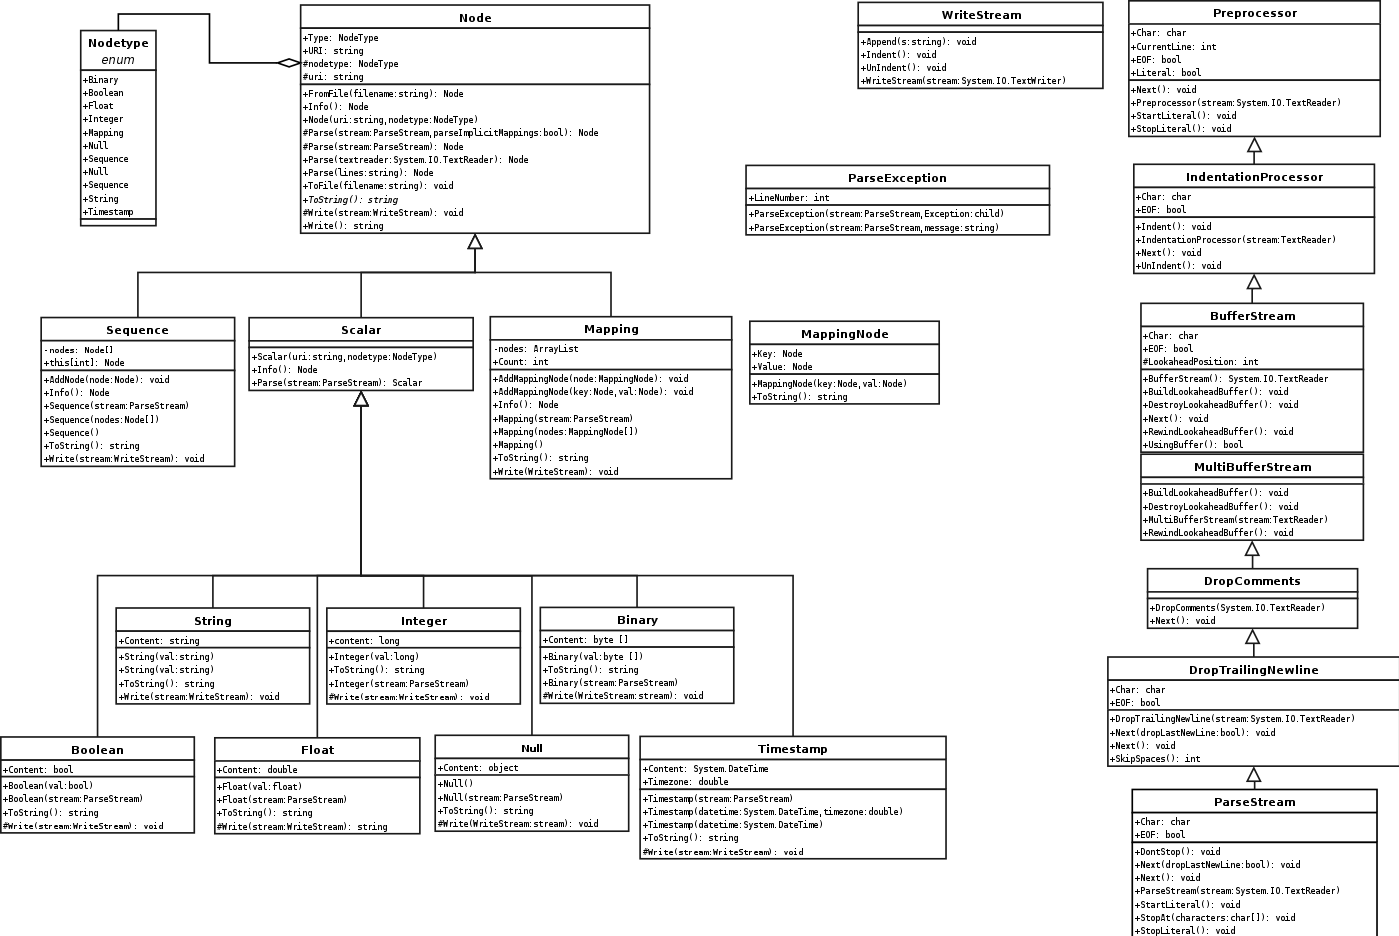
\includegraphics[width=1\textwidth]{uml.png}
	\caption{Definitieve UML diagram voor YAML .NET Parser (Grote versie in bijlage, blz. \pageref{fig:UMLDefLarge})}
	\label{fig:UMLDef}
\end{figure}
	% ---- ??
	\begin{analyse}
	Buiten de algemene boomstructuur merken we ook een \emph{stream} classe die eigenlijk de toegang is voor de gebruiker.
	Belangrijk is hierbij op te merken dat er zowel 'communicatie' mogelijk is via file I/O als via strings.
	
	Verder zijn de classe voor de test applicatie hier niet gerepresenteerd. Deze zullen minimaal van opbouw zijn en behoren
	strikt gezien ook niet tot de parser.
	\end{analyse}

	De \emph{parse stream} class is niet meer direct toegankelijk voor de gebruiker, deze moet nu enkel nog
	met de class \emph{node}, of een afgeleide class daarvan communiceren. De \emph{parse stream} vormt
	intern voor de parser een interface tot de stream, welke via een node zou kunnen zijn meegegeven om te
	parsen. De \emph{parse stream} voorziet verschillende transformaties die het parsen kunnen abstraheren.
	
	Een definitief UML diagram kan gevonden worden in figuur \ref{fig:UMLDef} en een grotere 
	versie in bijlage op blz. \pageref{fig:UMLDefLarge}.
	Bij de evaluatie van het Analyse verslag werden enkele suggesties gedaan die de structuur zouden
	kunnen verbeteren.

	De opmerking om de (Parse)Stream class afteleiden van IO.stream hebben we in overweging genomen. Maar gezien
	onze specifieke noden was dit niet voor de hand liggend. Wel is er voldoende compatibiliteit voorzien zodat van een
	StreamReader kan worden geparst.

	Verder heeft Jo ons een Set class aangeboden. Wegens het gebrek aan tijd hebben we deze niet nodig gehad.

	Er werd ons ook aangeraden de anchors in een aparte klasse te abstraheren. Daar we ook hier niet aan toe zijn gekomen
	zien we hier niets van terug in het definitieve UML diagram. Het is wel duidelijk dat er geen beperkingen zijn
	om dit later alsnog te doen.

	Tenslotte merken we enkele hulp classes op zoals \emph{ParseException} en \emph{Nodetype} die oorspronkelijk
	niet waren voorzien. De test classes waarover we sproken in het analyse verslag hebben we gegroepeerd
	onder de 'Examples'.

	\subsection{Verantwoording van de keuze van ADT's}

		\subsubsection{Algemene datastructuur}
		\begin{analyse}
		Onze datastructuur van een Yaml document zal uit een boom van nodes bestaan. De wortel
		is het Yaml document zelf, dit kan een mapping, sequence of scalar zijn. (Een bestand
		kan meerdere Yaml documenten bevatten, in dat geval hebben we een ArrayList\footnote{het
		.NET alternatief voor een vector} van documenten.

		Elk element wordt voorgesteld door een classe die van de class \emph{Node} erft. In het
		geval van een \emph{Mapping} zal elk item in een ArrayList opgeslagen worden waarbij
		voor elk item zowel een key als de data gespecifieerd worden. Zowel de key als de data
		kan eender welk type \emph{Node} zijn, zelfs een andere \emph{Mapping}.

		Een \emph{Sequence} zal ook opgeslagen worden als ArrayList, maar in dit geval is er
		enkel een value, ook van het type \emph{Node}. \emph{Scalars} zijn primaire types,
		de bladeren van de boom, deze erven wel van \emph{Node}, maar kunnen zelf geen kinderen
		hebben. We gaan verschillende klassen gebruiken die van \emph{Scalar} erven, om onder
		andere types zoals date, string en numerieke waarden te implementeren.
		\end{analyse}

	\subsection{Algoritmes}
		\begin{analyse}
		We zullen trachten een one-pass parser te maken, vermits bij het ontwerpen van Yaml hier
		extra aandacht aan besteed werd. Het maakt de implementatie misschien niet alleen
		eenvoudiger, maar ook sneller. De latere implementatie kan mogelijk afwijken omwille
		van een beter inzicht in de structuur die aantoont dat een ander algoritme effici\"enter
		is of meer volledig.
		\end{analyse}

		Onze parser is nog steeds zoals gepland een one-pass parser.

		\subsubsection{Enkele niveaus in de parse stream}

		De Parse stream heeft een gelaagde opbouw, elke laag bouwt verder op de vorige laag
		en voegt extra functionaliteit toe.

		\begin{enumerate}
		\item Preprocessor
		\item Indentatieprocessor
		\item Buffer
		\item Geneste buffer
		\item Comments verwijderen
		\item De laatste newline verwijderen
		\item Inline processor (Stopt op een gegeven karakter)
		\item Literal parsing (verbatim)
		\end{enumerate}

		De preprocessor houdt bij op welke regel dat we zitten, dit kan later gebruikt worden om
		bij het uitschrijven van een fout het regelnummer te vermelden. Voor het uitschrijven
		van fouten hebben we onze eigen Exception class voorzien.

		We gebruiken veel recursie om alles te parsen. Het tweede niveau, de indentatieprocessor,
		zorgt ervoor dat een genest of geindenteerd stuk Yaml net op dezelfde manier kan geparsed
		worden als een stuk code op het root-niveau.

		Onze parser is bijna volledig een one pass parser. We lezen van een stream en we bewegen
		ons enkel voorwaarts in de stream. Enkele Yaml structuren vereisen wel een beperkte vorm
		van lookahead. Soms moet parser even proberen of hij de volgende node als een bepaald
		type kan parsen, zo niet moet hij de buffer kunnen terugspoelen en een ander type
		proberen. Wij voorzien een circulaire buffer met een grootte van 1024 karakters wat
		volgens de documentatie is toegelaten. Omwille van de vaste buffergrootte en de werking
		van de buffer kunnen we de parser nog steeds een one-pass parser noemen.
	
		Soms hebben we zelfs een bufer nodig op een moment dat we al binnen een buffer aan het
		werken zijn. De vierde laag maakt geen buffer bij maar onthoudt de startpositie binnen
		de huidige buffer.

		We gebruiken een extra laag die de laatste newline verwijderd. Dit karakter behoort
		niet tot de content maar is enkel nodig omwille van de stuctuur waarmee Yaml is
		opgebouwd.

		Om eenvoudig inline structuren te parsen hebben we nog een extra laag toegevoegd.
		Hierin kan ingesteld worden dat op een bepaald karakter gestopt moet worden. Inline
		sequences bijvoorbeeld starten met een ''['' en eindigen met '']''.

		Strings die tussen enkele quotes staan moeten letterlijk genomen worden, dit houdt
		in dat newlines, tabs en spaties die hiertussen staan ook tot de werkelijke content
		van de string behoren. Het gedrag van de bovenliggende lagen moet ongedaan gemaakt
		worden. Dit gebeurt hier met de methoden StartLiteral en StopLiteral. Deze funtionaliteit
		is in werkelijkheid niet in een aparte laag geimplementeerd, maar wordt door de
		verschillende lagen geimplementeerd.

		We gebruiken veel samenhorende methoden, deze moeten altijd samen aangeroepen worden.
		Elke aanroep van Indent moet gepaard gaan met een latere aanroep van UnIndent,
		hetzelfde voor StopAt en DontStop, StartLiteral en StopLiteral.

		De meeste van deze lagen defini�ren de volgende functies:

		\begin{description}
		\item[Next] Ga naar het volgende karakter
		\item[Char] Geef het huidige karakter
		\item[EOF] (End of file) Geeft true terug indien we op 
								het einde van deze (deel)stream zitten.
		\end{description}

		\subsubsection{Indentatie processor}
		\begin{analyse}
		Indentatie is heel belangrijk in Yaml. Een regel die geen voorafgaande spaties heeft
		stelt een node voor, regels die volgen \'en meer ge\"indenteerd zijn dan de vorige regel,
		die zijn op de \'e\'en of andere manier geassocieerd met die node. Mogelijk vormen deze
		een blok dat een child van die node vormt. In dat geval zal de indentatie van deze child
		node verwijderd worden. Het aantal spaties dat verwijderd moet worden is het maximaal
		aantal spaties dat bij iedere regel van dat blok voorkomt, sommige regels zullen dus nog
		steeds voorafgaande spaties bevatten. Op een recursieve manier kunnen we nu dit blok parsen.
		\end{analyse}

		Dit is niet volledig waar. Enkel de eerste regel van een node bepaald hoeveel spaties
		deel uitmaken van de indentatie.

		We hebben twee belangrijke methoden: Indent en UnIndent. De eerste geeft aan dat
		we in een kind-node gaan welke waarschijnlijk maar niet noodzakelijk meer ge\"indenteerd
		is dan de parent node. Zoals ge�llustreerd in figuur \ref{fig:indent}.

\begin{figure}[h]
	\centering
	\begin{minipage}{2.5cm}
\begin{verbatim}
key:
  value
\end{verbatim}
	\end{minipage}
	\caption{Voorbeeld van indentatie \label{fig:indent}}
\end{figure}

		Bij het aanroepen van de \emph{Indent} functie - wat steeds gebeurt bij een overgang van
		parent naar child node - wordt een \emph{indentation-request} variabele geset. Wanneer we
		ons later verder verplaatsen in de stream en een newline karakter tegenkomen, dan gaan we
		naar de volgende regel en tellen het aantal indentatie karakters. Indien dit er meer zijn
		dan het aantal van de vorige regel, dan zitten we nog steeds in de child node. Zoniet
		(evenveel of minder indentatie), dan stopt hier het child blok en wordt EOF hier voorlopig
		op true gezet. Bij de aanroep van Indent wordt het huidige indentatie niveau op een stack
		geplaatst, zodat dit bij een \emph{UnIndent} terug kan worden hersteld. Het aanroepen van
		\emph{UnUndent} zal in indentation-request ongedaan maken indien we nooit een newline tegenkwamen,
		of anders het laatste indentatie niveau van de stack poppen. OEF wordt hierbij mogelijk ook
		terug of false geset.

		\subsubsection{De buffer}
		We gebruiken een circulaire buffer van \'e\'en kilochars. Een lookahead van meer dan 1024
		karakters is niet mogelijk, maar dit is niet vereist indien we de ristrictie kunnen opleggen
		dat een key van een impliciete mapping niet groter mag worden dan 1024. We hebben drie
		balangrijke integer variabelen: de rotatie, de positie en de grootte. De rotatie wijst naar
		de eerste cel van het stukje gebruikte buffer. Positie is de offset binnen dit stukje
		waar we momenteel aan het parsen zijn. Grootte is de grootte van dat stukje buffer.
		
		Wanneer we \emph{BuildLookaheadBuffer} aanroepen dan wordt de buffer geinitialiseerd, tenzij
		deze al eerder in gebruik was. Een \emph{DestroyLookaheadBuffer} verwijdert de buffer niet meteen
		maar gaat de buffer enkel alle karakters voor het huidige karakter laten vergeten. Hiermee
		kunnen we het toestaan om de destroy functie aan te roepen terwijl we nog midden in de buffer
		zitten. Na een aanroep van destroy zitten we nog steeds op hetzelfde karakter. Elke aanroep
		van Next zal telkens de positie pointer een plaats in de buffer doen opschuiven en weer het
		vorige karakter doen vergeten. Dit blijft zich herhalen totdat we aan het einde van de buffer
		komen en terug in de normale flow van de stream komen.

		Geneste buffers realiseren we door bij elke aanroep van BuildLookaheadBuffer de huidige
		positie op een stack te plaatsen indien de buffer al in gebruik was. Een rewind zal dan
		naar deze positie, en niet naar de allereerste positie springen. De Destroy functie zal
		de laatste positie van de stack poppen.

		\subsubsection{Inline processor}
		Een geopende accolade geeft het begin van een inline mapping aan. Als we vanaf daar verder
		willer parsen moet de recursieve functie die de childnode gaat parsen stoppen op een komma,
		wat het begin van een nieuw item is, maar ook aan bij de bijhorende gesloten accolade. Aan de
		functie \emph{StopAt} kunnen we een karakter array meegeven. Deze zal telkens dat we op
		\'e\'en van deze karakters komen de EOF op true plaatsen, totdat de \emph{DontStop} functie
		wordt aangeroepen. We gebruiken weer een stack om het gedrag van de parent te overschrijven.
		Hierbij is het ook mogelijk - in tegenstelling met het aanroepen van een Indent - om de
		stream te verlengen door bijvoorbeeld een leeg array mee te geven.

		\subsubsection{Het type node bepalen}
		\begin{analyse}
		Het herkennen van een sequence is eenvoudig omdat deze met een ``--'' (liggend streepje of dash) begint.
		Een mapping bevat altijd een ``:'' (dubbele punt). In moeilijke gevallen (Bijvoorbeeld wanneer de key zelf
		een mapping is) wordt de key door een ``?'' (vraagteken) voorafgegaan wat het parsen vereenvoudigt. Voor het
		parsen is nog niet bekend om welk type node het gaat, dus indien dit geen mapping of sequence is, kan het
		net zo goed nog een scalar zijn.
		\end{analyse}

		Bepaalde types van nodes kunnen we al onmiddellijk aan de eerste karakters herkennen.
		Bij nodes die beginnen met twee uitroeptekens gevolgd door de typenaam kan meteen de
		parse functie van dat type nood aangeroepen worden. Het liggend streepje aan het
		begin duidt op het volgen van een sequence, net zoals een vraagteken wijst op een mapping.
		Andere types vereisen lookahead door middel van een buffer. Verder wijzen een open
		accolade of vierkantig haakje op respectievelijk een inline mapping en inline sequence.

		Het eerste wat we nu moeten controleren zijn inline mappings. De enige manier waar deze
		aan te herkennen zijn is de dubbele punt die na de eerstvolgende scalar volgt. Dit houdt
		in dat we eerst deze scalar moeten parsen, en daarna zien of er een dubbele punt volgt.
		Volgt er geen dubbele punt, dan moeten we terugspoelen tot voor deze scalar en terug alle
		soorten scalars uitproberen.


		\subsubsection{Scalars}
		\begin{analyse}
		Indien na het parsen van de structuur bekend is dat een bepaald stukje tekst een scalar
		voorstelt, moet dit geparst worden. Hiervoor hebben we een methode in de class \emph{scalar}
		die bepaalt om welk type scalar het gaat (datum, float, ...), en daarna een instantie van
		de gepaste subclass teruggeeft.

		Veel kan al bepaald worden door het eerste karakter. Scalars die met een enkele
		quote --- ' --- beginnen zijn ongeescapete strings, een dubbele quote --- '' --- geeft het
		begin aan van een geescapte string. ''$>$'' en ''$|$'' zijn het begin van respectievelijk
		een \emph{folded block} en een \emph{literal block}. (Een folded block is een blok waar
		regeleindes door spaties vervangen worden.) Andere scalars kunnen eenvoudig met reguliere
		expressies herkend worden.
		\end{analyse}
		
		Bij het parsen van scalars wordt intensief gebruik gemaakt van de voorziene buffer uit
		de \emph{ParseStream}. Een uitzondering hierop is indien er gebruik wordt gemaakt van tags
		zoals \emph{!!str}, \emph{!!float}, \ldots, dan was al eerder bekend om welk type het gaat.
		We proberen telkens een bepaald type, indien deze node niet geldig is volgens dat type,
		wordt er een error geworpen die maakt dat we het volgende type proberen. Als laatste wordt
		het type string geprobeerd omdat bijna alles als geldige string kan worden geinterpreteerd.
		Er is ook ondersteuning voor folded en literal blocks, maar deze zijn nog niet volledig;
		onderandere $+$ en $-$ chomps zijn niet ondersteund.
		
		Volgende scalars worden ondersteund:
		\begin{enumerate}
			\item Strings
			\item Booleans
			\item Null values
			\item Integers
			\item Floats
			\item Timestamps
			\item Binary data
		\end{enumerate}
		
		Scalars worden niet gemapped op native C\# datatypes zoals we zouden doen bij het echt
		(de)serialiseren via reflectie. Wij gebruiken de native types wel, maar deze steken we
		telkens in een eigen container afgeleid van een node. Hierdoor is het eenvoudig deze in
		boomstucturen als mappings en sequences te steken. Timestamps zijn een geval apart;
		Yaml biedt de mogelijkheid om een tijdzone te defini�ren, maar dit is niet aanwezig in
		de 1.0 versie van .NET. Daarom komen we niet toe met het native datatype alleen en hebben
		we een extra variabele om de tijdzone te bewaren opgeslagen.
		
		Bij het parsen van de scalars hebben we het gebruik van reguliere expressies vermeden.
		Aangezien we een one-pass parser hebben trachten te implementeren was het logisch om
		geen reguliere expressies te gebruiken. Ook zouden reguliere expressies de effici�ntie
		niet ten goede komen in ons geval.
		
		\subsubsection{Ordered maps, pairs en sets}
		\begin{analyse}
		Dit zijn datastructuren die van sequences en mappings afgeleid zijn. Ordered maps en
		pairs worden voorgesteld door een sequence van maps, het verschil is dat bij pairs wel
		duplicaten worden toegelaten en bij ordered maps niet. Sets worden voorgesteld als
		mappings waarbij de value telkens gelijk is aan nul.
		\end{analyse}

		Zoals reeds eerder aangehaald bij het bespreken van het klasse-diagram (sectie \ref{UMLDef})
		hebben we deze functionaliteit niet ge�mplementeerd. Het aanbieden van deze structuren aan de
		parser geeft geen problemen aangezien we deze mappen op de reeds ge�mplementeerde types.
		
		Momenteel worden sets nog als normale mappings gezien bestaande uit keys zonder value, maar
		deze constraint wordt nog niet gecontroleerd. Op dezelde manier worden pairs geparsed als
		sequences zonder de pair-specifieke constraints te controleren.

		\subsubsection{Integratie van het .NET Framework}
		\begin{analyse}
		Na het parsen verkrijgen we een boom die opgebouwd is uit onze eigen datatypes, dit in
		tegenstelling tot sommige implementaties (Ruby) waar dat de 'native' datatypes van de
		taal gebruikt worden. Het voordeel van de tweede methode is dat dit het gebruik van de
		library volledig transparant maakt. De gebruiker hoeft niet meer te weten dan de syntax
		van de parse en write functies en kan verder werken met de standaard datatypes zoals
		arrays en hashes welke in de taal geimplementeerd zijn. We onderzoeken nog in hoeverre
		deze manier van werken mogelijk zal zijn voor .NET.
		\end{analyse}

		We zijn bij ons eerste idee gebleven om eigen wrapper classes te implementeren voor de
		verschillende datatypes.

		De class Node heeft een statische \emph{Parse} functie die een stream of string meekrijgt
		en \'e\'en van zijn kinderen teruggeeft afhankelijk van het type node. De \emph{Write}
		functie van node maakt van een node terug een Yaml string en de \emph{ToString} functie
		geeft de inhoud in string vorm terug. Deze laatste dient enkel om eenvoudig te controleren
		of Yaml code daadwerkelijk juist wordt geparsed.
		
		\begin{analyse}
		Het zal niet vanzelfsprekend zijn (misschien onmogelijk) om de inhoud van een willekeurige
		class uit te schrijven naar een Yaml stream. Ruby, python, perl en PHP zijn scriptingtalen,
		welke flexibele mogelijkheden ondersteunen voor het het omgaan met datatypes.
		\end{analyse}

		Bij het bespreken van het analyse verslag werd het gebruik van reflection besproken. Dit zou
		een gedeeltelijke oplossing kunnen zijn. Wegens gebrek aan tijd en ervaring op dat gebied
		zien we hier niet aan toe kunnen komen.

	\section{Het programmeren}
	Aanvankelijk was C\# voor Christophe een nieuwe programmeertaal. Het was een motivatie om dit
	project te doen, omdat we op deze manier iets nieuw konden leren. 

	Als referentie hebben we \cite{MSDN}, \cite{insidecsharp} en \cite{csharppro} gebruikt. In 
	mindere maten hebben we ook de website van het Mono Project geraadpleegd \cite{Mono}.
	Ook de hulp van Gert van Gool en Ingo Berben stellen we erg op prijs. Ook zij hebben hun trimester 
	overschreidend project gemaakt in C\# wat zorgde voor een interessante wisselwerking.

	\subsection{Probleempjes}
	Tijdens het programmeren hebben we geen spectaculaire problemen gehad. Enkele puntjes die we hier misschien
	willen aanhalen zijn het boxing en unboxing probleem en het omgaan met binaire data.

	Op een gegeven moment wenste we een \emph{int} als parameter mee te geven als een reference. Dit bleek echter
	niet te lukken We hebben hier boxing en unboxing voor trachten te gebruiken, wat niet het gewenste effect gaf.
	Het gebruik van pointers wordt in C\# wordt afgeraden, maar we vonden de \emph{out} constuctie waarmee we
	functie parameters konden veranderen.

	Ook hebben we ons verdiept in een nieuw aspect, binaire data. Zo wordt binaire data in
	Yaml gerepresenteerd in Base64. Afhankelijk wilde we dit volledig zelf gaan parsen.
	Echter met het gebruik van de juiste library \emph{System.Convert} is het relatief
	eenvoudig. Deze voorziet ook in de functionaliteit om een byte array terug om te zetten
	naar Base64.

	Aangezien ons project intensief steunt op het appenden van string hebben we gebruik gemaakt
	van \emph{System.Text.StringBuilder}. Dit is efficienter dan rechtstreeks op een string
	te werken aangezien er bij elke wijziging van een gewone string steeds een nieuwe instantie
	wordt gecre\"erd.

	Vaak hebben we problemen gahad dat nieuwe code interfereerde met al eerder geschreven code. Door
	alles goed op splitsen zijn de meeste problemen verholpen.

	We hebben nog enkele Yaml specifieke problemen. De integer \emph{-1} wordt als een sequence gezien
	omdat we de spatie na het liggend streepje nog niet verplichten. \emph{!!int -1} gebruiken is
	voorlopig een oplossing. Een ander gelijkaardig probleem hebben we bij timestamps: \emph{2006-06-01 8:45}
	hier wordt de dubbele punt als mapping gezien, tenzij de timestamp door een \emph{!!timestamp} tag
	voorafgegaan wordt.
	
	\subsection{Library}
	Het is logisch dat ons project als library werd gepubliceerd. In plaats van een normale executable 
	file voorzien wij in een DLL file. In het vak \emph{Geavanceerde programmeer technieken} zijn 
	de technieken voor het maken van libraries uitgelegd voor C en C++. In het .NET platform
	zijn enkele zaken vereenvoudigd en is er rekening gehouden met de problemen uit het verleden.
	Zo wordt de developper gemotiveerd om zijn code te \emph{signen}. Het heeft ons enig zoekwerk gekost,
	maar uiteindelijk hebben we deze redelijk eenvoudige klus toch geklaard.
	
\section{Open Source}
Zoals beloofd publiceren we ons project als Open Source. We waren hier niet vertrouwt mee
maar gelukkig zijn we hier goed in geholpen. We hebben nauwgezet de richtlijnen van 
de GPL \cite{GPL} website gevolgd \footnote{Het onderwijsteam was bij het ter perse gaan van dit 
verslag nog bezig met het verzorgen van de nodige gegevens betreffende de 'supporting school'. 
Uiteraard wordt dit aangepast zodra dit bekend is.}.
We hebben verder ook gekozen om de Lesser GPL 
licentie te gebruiken. Dit geeft de mogelijkheid om de library te gebruiken in commerci�le 
pakketten, op voorwaarde dat de library vrij beschikbaar blijft.

\section{Taakverdeling en planning}

%Een eerste zaak zal zijn om ons zelf vertrouwd te maken met Yaml en de manier waarop we dit soort documenten kunnen parsen.
%Dit zal vooral inhouden de specificaties en beschikbare documentatie verder door te nemen.
%Verder zal Christophe zich ook eigen moeten maken aan de taal C\#, Jonathan heeft hier reeds ervaring mee.
%
%Aangezien het tweede trimester voor meer dan 50\% is gevorderd zal het schrijven van code en testen voornamelijk gebeuren
%in de Paasvakantie en het begin van het derde trimester. Tenslotte rest ons nog de documentatie en presentatie. 

	\begin{analyse}
	Dit trimester hopen we nog voldoende research te kunnen doen. Verder trachten we ook in
	communicatie te gaan met de hoofdleden en community van Yaml. Enerzijds om hen te informeren
	rond ons project en anderzijds eventuele ondersteuning te verkrijgen.
	\end{analyse}

	Ons verdiepen in Yaml (en C\#) heeft zoals gepland het volledige tweede trimester ingenomen. We
	hebben enige test code geschreven en heel beperkt de Ruby parser bestudeerd. Achteraf bekeken was
	het niet nodig de Yaml specificatie zo diepgaand te bestuderen aangezien we slecht een beperkt deel
	hebben geimplementeerd. Het had misschien verstandiger geweest om sneller te beginnen programeren
	en indien nodig later de Yaml documentatie terug ter hand te nemen. De vraag die we ons kunnen
	stellen is echter of we dan geen cruciale fouten hadden gemaakt in onze structuur?

	We hebben in de laatste week van het project onze parser aangekondigd op de Yaml mailing list. We
	dachten hier heel wat reacties op te ontvangen, dit is spijtig genoeg niet het geval. Onze algemene
	indruk is dat Yaml communitie aan het stilvallen is. In het begin van het project waren er hevige
	discussies, nu wordt er slechts sporadisch gepost.

	\begin{analyse}
	Onze Yaml parser zal zoals eerder gezegd een one-pass parser worden, we kunnen dus geen taakverdeling
	maken op basis van de passes. Een goede verdeling is dat \'e\'en iemand de individuele scalars gaat
	parsen en iemand anders de grotere structuren zoals sequences en mappings. Voor we dit kunnen beslissen
	moeten we ons beide verdiepen in de details van Yaml, dit is iets dat we niet kunnen opdelen. Tenslotte
	zal afhankelijk van wie het verst gevorderd is bepaald worden wie de Yaml generator gaat schrijven.
	Als tegen gewicht op de Yaml generator zijn er nog talloze andere hulp functies nodig, die dan de
	andere persoon voor zijn rekening kan nemen.
	\end{analyse}

	In het analyse verslag hadden we slecht een beperkt idee van de taakverdeling. We hebben wel op
	aanraden van het onderwijsteam getracht een duidelijkere taakverdeling te maken. Van de moment dat
	we zijn beginnen programmeren hebben we de Yaml structuur in twee delen opgedeeld. Enerzijds de
	Collection types (mappings, sequence, \ldots) en anderzijds de Scalar types. Aangezien de Scalar
	types aanvankelijk eenvoudig leken heeft Christophe dit voor zijn rekening genomen. Volgens de
	oorspronkelijke planning zou dit niet de volledige ontwikkelingstijd innemen en zou er zo
	een reserve zijn om aan andere delen of extra's te werken. Dit is echter niet gelukt en zo heeft
	Jonathan zowel de Collections types als de onderliggende stream structuur uitgewerkt.

	Een overzicht van onze logs is te vinden in bijlage \ref{logs}, blz. \pageref{logs}.

\section{Slot opmerking}

	\begin{analyse}
	Het is duidelijk dat dit geen standaard project zal worden. Dit is ook onze belangrijkste
	motivatie om te kiezen voor iets wat we nog niet kennen en hopelijk veel van kunnen bijleren.
	We verwachten ons aan moeilijke momenten en gaan ervan uit dat niet alles even vlot zal
	verlopen als we willen. We hopen dat we kunnen rekenen op de nodige steun van uit het onderwijs team.
	\end{analyse}

	\subsection{Ons standpunt t.o.v. Yaml}
	Yaml is goed leesbaar en verstaanbaar. Verder is het ook eenvoudig om te schrijven, maar naar
	onze mening heeft de gebruiker te veel vrijheid. Zo kunnen dezelfde dingen op verschillende
	manieren worden geschreven. Dit resulteert in meer verwarring dan dat het helpt. We zijn het
	dan ook volledig eens met de communitie dat er een vereenvoudiging van Yaml nodig is.

	Yaml is een mooi alternatief voor XML. Het grote voordeel van Yaml is de ondersteuning voor
	ankers en referenties. Dit maakt, buiten boomstructuren, ook circulaire en accyclische
	datastructuren mogelijk.

	Yaml moet vooral nog heel hard groeien! (Of inkrimpen?)

	\subsection{Het project in het algemeen}

	Zoals verwacht hebben we veel bijgeleerd. We hebben tot onze verbazing nooit de hulp
	van het onderwijs team moeten inroepen. Yaml en C\# zijn dan ook twee heel toegankelijke
	items die met een beetje doorzettings vermogen goed te verwerken zijn.

\appendix

\section{Bijlage}

\subsection{UML Diagram}
\label{fig:UMLDefLarge}
	
\begin{figure}[H]
	\centering
		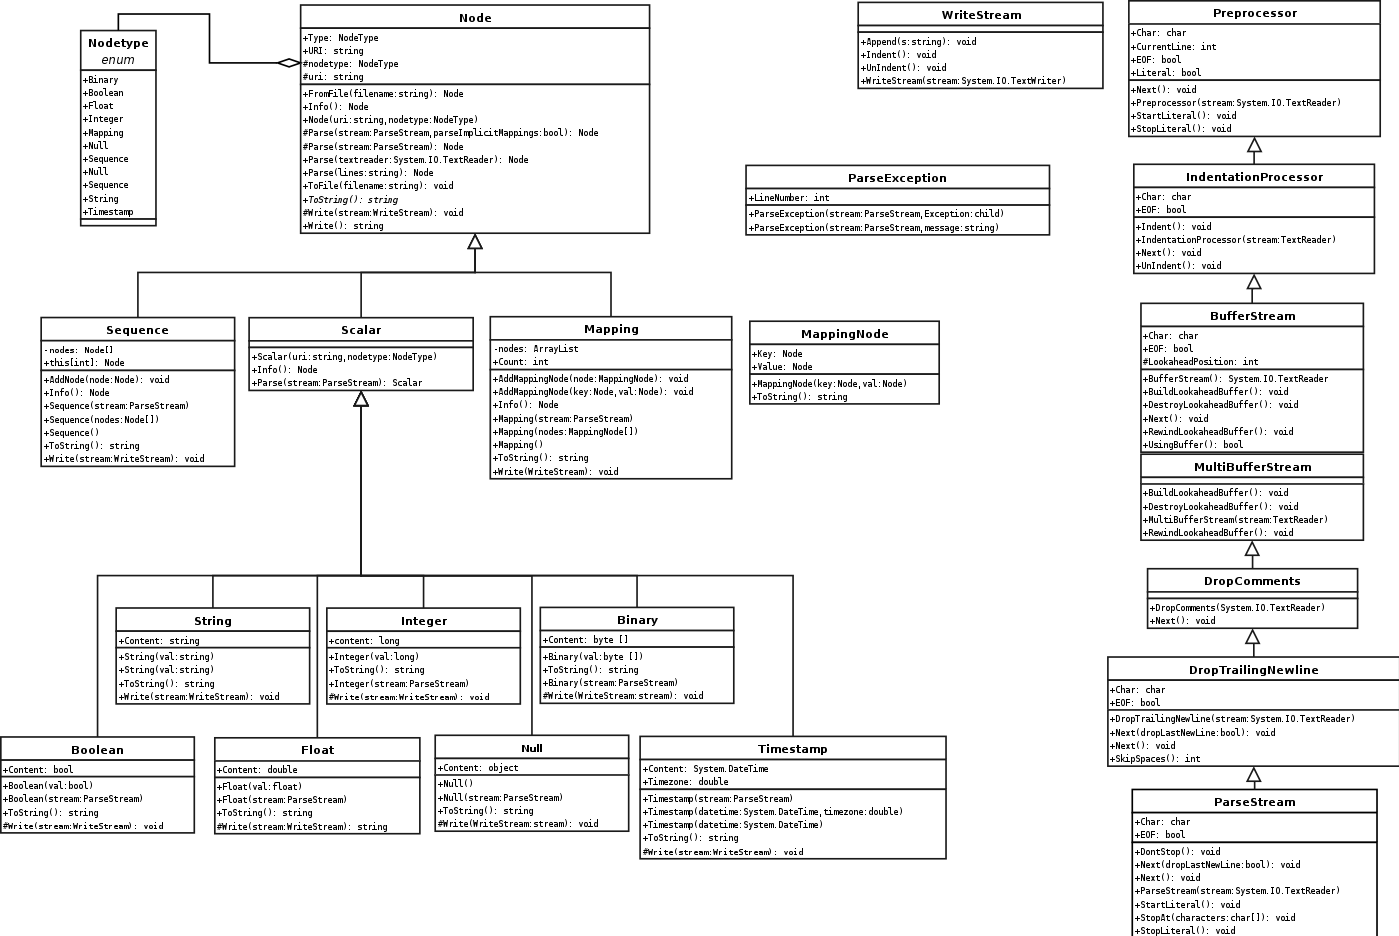
\includegraphics[angle=90,width=1\textwidth]{uml.png}
\end{figure}

\subsection{Logs in Yaml}
\label{logs}

\subsubsection{Jonathan Slenders}
\verbatiminput{../Log_Jonathan.yaml}

\subsubsection{Christophe Lambrechts}
\verbatiminput{../Log_Christophe.yaml}

\subsection{Onderinge communicatie in Yaml}
\label{chat}

%Yaml chat invoegen
\verbatiminput{../Chat.yaml}

\subsection{Manual}

Voor een actuele versie van de manual verwijzen we naar de project website op
\url{http://lumumba.uhasselt.be/\~christophe/YAML/}. We voegen hier een versie toe
van 8 juni 2006.

%Outprint van website, hier invoegen
\newpage

\bibliographystyle{plain}
\bibliography{bibliografie}
\footnotetext{Bij het ter perse gaan van dit eind verslag zijn alle URL's voor een laatste maal bezocht en geverifieerd.}

\end{document}
